\documentclass[a4paper, 11pt]{article}
\usepackage{amsmath}
\usepackage{graphicx}
\usepackage{tikz}
\usepackage[hidelinks]{hyperref}
\usepackage{color}
\usepackage{xcolor}
\usepackage{listings}

\lstset{basicstyle=\small}

\usepackage{caption}
\DeclareCaptionFont{white}{\color{white}}
\DeclareCaptionFormat{listing}{\colorbox{gray}{\parbox{\textwidth}{#1#2#3}}}
\captionsetup[lstlisting]{format=listing,labelfont=white,textfont=white}

\begin{document}
%Header-Make sure you update this information!!!!
\noindent
\large\textbf{Obligatory Assignment 1 Report} \hfill \textbf{Tomasz Gliniecki} \\

\section*{Problem Statement}
\subsection*{Monty Hall problem}
When a contestant is to choose one of three gates, where behind one of them is a prize, one can choose strategy as a result of the rules of the game. After the initial choice of the gate one ot the remaining gates that \emph{has no car behind it} gets reveiled. Now the strategy is either to keep the initial gate or switch.\cite{montyhall}\\
The most effective strategy \emph{in the long run} is to ALWAYS SWITCH. This is because, one has always $\frac{2}{3}$ chance of winning by swithcing. This is obvoius because, there is $\frac{1}{3}$ chance of finding the prize which is behind 1 of the 3 gates, that means that there is $\frac{2}{3}$ chance of NOT finding the prize. If we set our goal to NOT find the prize, and then switch when the empty gate opens, we will win with a $\frac{2}{3}$ probability, because there is $\frac{2}{3}$ chance of not finding the prize!\\
The simulation from [Listing \ref{lst:keepmonty}] shows that there is approximately $ ~[1] 0.6771 $ chance of winning with strategy 2.

\subsection*{Rock Paper Scissors}
There is $\frac{1}{3}$ chance of choosing either of the shapes. Probability for a person to NOT choose "rock" is $\frac{2}{3}$ because then it's either "paper" or "scissors". Whatever the eperson chooses has no influence on what the other chooses, that means there is $\frac{2}{3}$ chance for one person to not choose whatever the other person choose, thus giving $\frac{2}{3}$ chance for the game to end successfully. If on the other hand we look at the possibility to end the game in a tie, it is clearly $\frac{1}{3}$ because if we look at the possibility to choose "rock", then its abviously $\frac{1}{3}$, if one person will choose rock independently the other has $\frac{1}{3}$ chance of doing the same.\\
The expected number of trials until there is a winner is:
$ 1/\frac{2}{3}  $\\
The results of k = 1 from the simulation is very close to $ 1/\frac{2}{3} =1.5 $
\begin{center}
  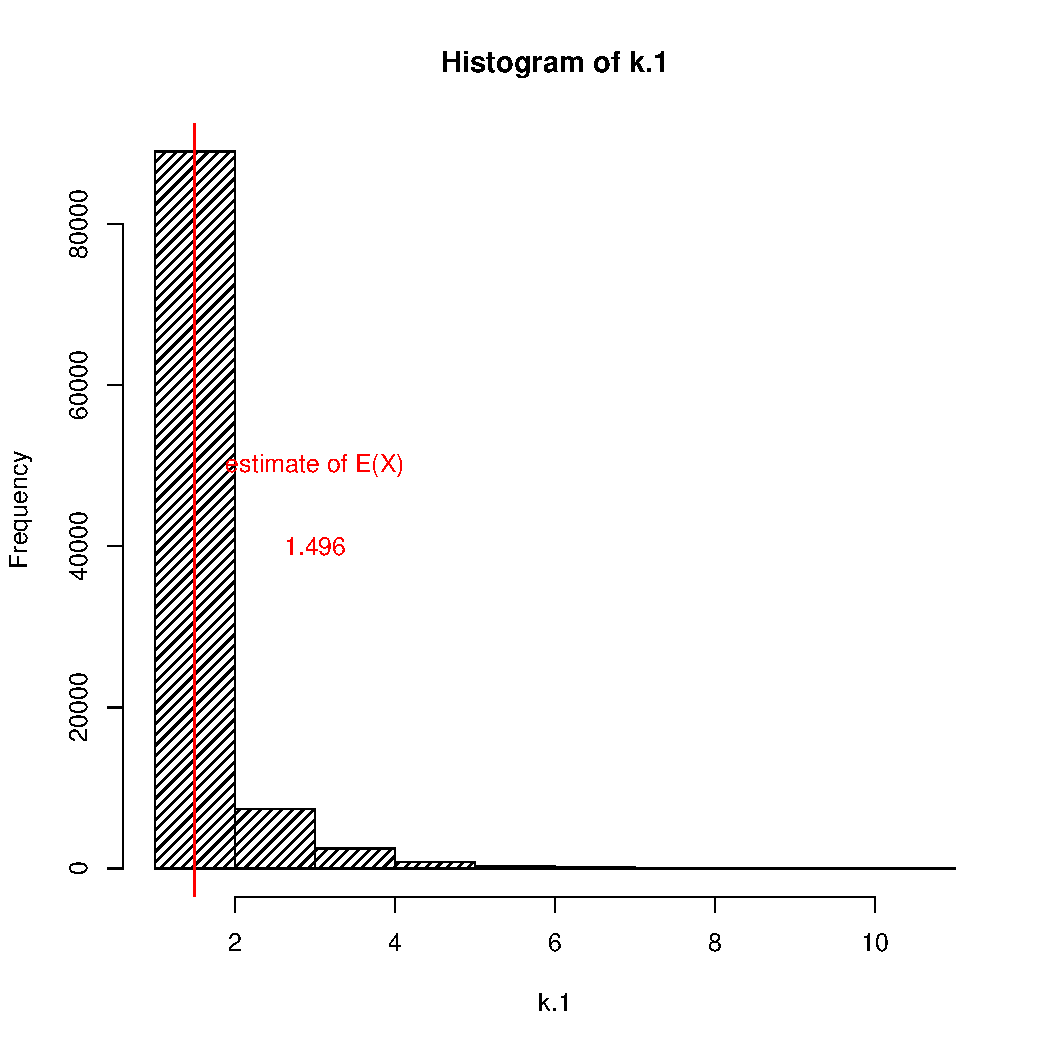
\includegraphics[scale=0.7,page=1]{Rplots.pdf}
\end{center}

\newpage
The estimatet number of trials untill there is a winner after $10^5$ simulations is as follows:

\begin{center}
  \includegraphics[scale=0.7,page=2]{Rplots.pdf}
\end{center}
\begin{center}
  \includegraphics[scale=0.7,page=3]{Rplots.pdf}
\end{center}
\section*{Solutions}

\newpage
\section*{Construction/Implementation}
\begin{lstlisting}[caption={Simulation of "swtich" strategy in Monty Hall problem},label={lst:keepmonty},language=R]
for (i in c(0:1e4)) {
  gate_distribution <- sample(possible_items, prob=c(1/3,1/3,1/3));
  contestant_choice <- sample(possible_choices,size=1,prob=c(1/3,1/3,1/3));
  # amount of wins strategy 2
  if (``car'' %in% gate_distribution[-contestant_choice]) {
  switch <- switch+1;
  }
}
\end{lstlisting}

\begin{lstlisting}[caption={Number of trials needed to finish the game given k lives},label={lst:ntrials},language=R]
play_rps <- function(lives=1) {
  k <- 0;
  while(1) {

    #independent choices
    player0 <- sample(elements,size=1,prob=p);
    player1 <- sample(elements,size=1,prob=p);

    ifelse ((player0==''R'' && player1==''S''), p0win <- p0win+1,
    ifelse ((player0==''R'' && player1==''P''), p1win <- p1win+1,

    ifelse ((player0==''P'' && player1==''R''), p0win <- p0win+1,
    ifelse ((player0==''P'' && player1==''S''), p1win <- p1win+1,

    ifelse ((player0==''S'' && player1==''P''), p0win <- p0win+1,
    ifelse ((player0==''S'' && player1==''R''), p1win <- p1win+1,NA))))));

    k <- k+1;

    if (p0win>=lives || p1win>=lives) {
      break
    }
  }

  return(k);
}
\end{lstlisting}


\section*{Attachments}

montyhallproblem.R rps.R Rplots.pdf

\begin{thebibliography}{9}
  
\bibitem{montyhall} 
  Monty Hall problem, [cited 27.September 2016]. Available at \url{https://en.wikipedia.org/wiki/Monty_Hall_problem}

\end{thebibliography}

\end{document}
